%%% The main file. It contains definitions of basic parameters and includes all other parts.

%% Settings for single-side (simplex) printing
% Margins: left 40mm, right 25mm, top and bottom 25mm
% (but beware, LaTeX adds 1in implicitly)
\documentclass[12pt,a4paper]{report}
\setlength\textwidth{145mm}
\setlength\textheight{247mm}
\setlength\oddsidemargin{15mm}
\setlength\evensidemargin{15mm}
\setlength\topmargin{0mm}
\setlength\headsep{0mm}
\setlength\headheight{0mm}
% \openright makes the following text appear on a right-hand page
\let\openright=\clearpage

%% Settings for two-sided (duplex) printing
% \documentclass[12pt,a4paper,twoside,openright]{report}
% \setlength\textwidth{145mm}
% \setlength\textheight{247mm}
% \setlength\oddsidemargin{14.2mm}
% \setlength\evensidemargin{0mm}
% \setlength\topmargin{0mm}
% \setlength\headsep{0mm}
% \setlength\headheight{0mm}
% \let\openright=\cleardoublepage

%% Generate PDF/A-2u
\usepackage[a-2u]{pdfx}

%% Character encoding: usually latin2, cp1250 or utf8:
\usepackage[utf8]{inputenc}

%% Prefer Latin Modern fonts
\usepackage{lmodern}

%% Further useful packages (included in most LaTeX distributions)
\usepackage{amsmath}        % extensions for typesetting of math
\usepackage{amsfonts}       % math fonts
\usepackage{amsthm}         % theorems, definitions, etc.
\usepackage{bbding}         % various symbols (squares, asterisks, scissors, ...)
\usepackage{bm}             % boldface symbols (\bm)
\usepackage{graphicx}       % embedding of pictures
\usepackage{fancyvrb}       % improved verbatim environment
\usepackage{natbib}         % citation style AUTHOR (YEAR), or AUTHOR [NUMBER]
\usepackage[nottoc]{tocbibind} % makes sure that bibliography and the lists
			    % of figures/tables are included in the table
			    % of contents
\usepackage{dcolumn}        % improved alignment of table columns
\usepackage{booktabs}       % improved horizontal lines in tables
\usepackage{paralist}       % improved enumerate and itemize
\usepackage[usenames]{xcolor}  % typesetting in color

%%% Basic information on the thesis

% Thesis title in English (exactly as in the formal assignment)
\def\ThesisTitle{Genres classification by means of machine learning}

% Author of the thesis
\def\ThesisAuthor{Bc. Jan Bílek}

% Year when the thesis is submitted
\def\YearSubmitted{2018}

% Name of the department or institute, where the work was officially assigned
% (according to the Organizational Structure of MFF UK in English,
% or a full name of a department outside MFF)
\def\Department{Department of Theoretical Computer Science and Mathematical Logic}

% Is it a department (katedra), or an institute (ústav)?
\def\DeptType{Department}

% Thesis supervisor: name, surname and titles
\def\Supervisor{Mgr. Roman Neruda Csc.}

% Supervisor's department (again according to Organizational structure of MFF)
\def\SupervisorsDepartment{Institute of Computer Science, The Czech Academy of Sciences}

% Study programme and specialization
\def\StudyProgramme{Computer Science}
\def\StudyBranch{Artificial Intelligence}

% An optional dedication: you can thank whomever you wish (your supervisor,
% consultant, a person who lent the software, etc.)
\def\Dedication{%
Dedication.
}

% Abstract (recommended length around 80-200 words; this is not a copy of your thesis assignment!)
\def\Abstract{%
Abstract.
}

% 3 to 5 keywords (recommended), each enclosed in curly braces
\def\Keywords{%
{key} {words}
}

%% The hyperref package for clickable links in PDF and also for storing
%% metadata to PDF (including the table of contents).
%% Most settings are pre-set by the pdfx package.
\hypersetup{unicode}
\hypersetup{breaklinks=true}

% Definitions of macros (see description inside)
%%% This file contains definitions of various useful macros and environments %%%
%%% Please add more macros here instead of cluttering other files with them. %%%

%%% Minor tweaks of style

% These macros employ a little dirty trick to convince LaTeX to typeset
% chapter headings sanely, without lots of empty space above them.
% Feel free to ignore.
\makeatletter
\def\@makechapterhead#1{
  {\parindent \z@ \raggedright \normalfont
   \Huge\bfseries \thechapter. #1
   \par\nobreak
   \vskip 20\p@
}}
\def\@makeschapterhead#1{
  {\parindent \z@ \raggedright \normalfont
   \Huge\bfseries #1
   \par\nobreak
   \vskip 20\p@
}}
\makeatother

% This macro defines a chapter, which is not numbered, but is included
% in the table of contents.
\def\chapwithtoc#1{
\chapter*{#1}
\addcontentsline{toc}{chapter}{#1}
}

% Draw black "slugs" whenever a line overflows, so that we can spot it easily.
\overfullrule=1mm

%%% Macros for definitions, theorems, claims, examples, ... (requires amsthm package)

\theoremstyle{plain}
\newtheorem{thm}{Theorem}
\newtheorem{lemma}[thm]{Lemma}
\newtheorem{claim}[thm]{Claim}

\theoremstyle{plain}
\newtheorem{defn}{Definition}

\theoremstyle{remark}
\newtheorem*{cor}{Corollary}
\newtheorem*{rem}{Remark}
\newtheorem*{example}{Example}

%%% An environment for proofs

%%% FIXME %%% \newenvironment{proof}{
%%% FIXME %%%   \par\medskip\noindent
%%% FIXME %%%   \textit{Proof}.
%%% FIXME %%% }{
%%% FIXME %%% \newline
%%% FIXME %%% \rightline{$\square$}  % or \SquareCastShadowBottomRight from bbding package
%%% FIXME %%% }

%%% An environment for typesetting of program code and input/output
%%% of programs. (Requires the fancyvrb package -- fancy verbatim.)

\DefineVerbatimEnvironment{code}{Verbatim}{fontsize=\small, frame=single}

%%% The field of all real and natural numbers
\newcommand{\R}{\mathbb{R}}
\newcommand{\N}{\mathbb{N}}

%%% Useful operators for statistics and probability
\DeclareMathOperator{\pr}{\textsf{P}}
\DeclareMathOperator{\E}{\textsf{E}\,}
\DeclareMathOperator{\var}{\textrm{var}}
\DeclareMathOperator{\sd}{\textrm{sd}}

%%% Transposition of a vector/matrix
\newcommand{\T}[1]{#1^\top}

%%% Various math goodies
\newcommand{\goto}{\rightarrow}
\newcommand{\gotop}{\stackrel{P}{\longrightarrow}}
\newcommand{\maon}[1]{o(n^{#1})}
\newcommand{\abs}[1]{\left|{#1}\right|}
\newcommand{\dint}{\int_0^\tau\!\!\int_0^\tau}
\newcommand{\isqr}[1]{\frac{1}{\sqrt{#1}}}

%%% Various table goodies
\newcommand{\pulrad}[1]{\raisebox{1.5ex}[0pt]{#1}}
\newcommand{\mc}[1]{\multicolumn{1}{c}{#1}}


% Title page and various mandatory informational pages
\begin{document}
%%% Title page of the thesis and other mandatory pages

%%% Title page of the thesis

\pagestyle{empty}
\hypersetup{pageanchor=false}
\begin{center}

\centerline{\mbox{
\includegraphics[width=166mm]{img/logo-en.pdf}}}

\vspace{-8mm}
\vfill

{\bf\Large MASTER THESIS}

\vfill

{\LARGE\ThesisAuthor}

\vspace{15mm}

{\LARGE\bfseries\ThesisTitle}

\vfill

\Department

\vfill

\begin{tabular}{rl}

Supervisor of the bachelor thesis: & \Supervisor \\
\noalign{\vspace{2mm}}
Study programme: & \StudyProgramme \\
\noalign{\vspace{2mm}}
Study branch: & \StudyBranch \\
\end{tabular}

\vfill

% Zde doplňte rok
Prague \YearSubmitted

\end{center}

\newpage

%%% Here should be a bound sheet included -- a signed copy of the "bachelor
%%% thesis assignment". This assignment is NOT a part of the electronic
%%% version of the thesis. DO NOT SCAN.

%%% A page with a solemn declaration to the bachelor thesis

\openright
\hypersetup{pageanchor=true}
\pagestyle{plain}
\pagenumbering{roman}
\vglue 0pt plus 1fill

\noindent
I declare that I carried out this bachelor thesis independently, and only with the cited
sources, literature and other professional sources.

\medskip\noindent
I understand that my work relates to the rights and obligations under the Act No.~121/2000 Sb.,
the Copyright Act, as amended, in particular the fact that the Charles
University has the right to conclude a license agreement on the use of this
work as a school work pursuant to Section 60 subsection 1 of the Copyright Act.

\vspace{10mm}

\hbox{\hbox to 0.5\hsize{%
In ........ date ............	% FIXME!
\hss}\hbox to 0.5\hsize{%
signature of the author
\hss}}

\vspace{20mm}
\newpage

%%% Dedication

\openright

\noindent
\Dedication

\newpage

%%% Mandatory information page of the thesis

\openright

\vbox to 0.5\vsize{
\setlength\parindent{0mm}
\setlength\parskip{5mm}

Title:
\ThesisTitle

Author:
\ThesisAuthor

\DeptType:
\Department

Supervisor:
\Supervisor, \SupervisorsDepartment

Abstract:
\Abstract

Keywords:
\Keywords

\vss}

\newpage

\openright
\pagestyle{plain}
\pagenumbering{arabic}
\setcounter{page}{1}


%%% A page with automatically generated table of contents of the bachelor thesis

\tableofcontents

%%% Each chapter is kept in a separate file
%\include{preface}
\chapter{Introduction}

Approx. two pages wrappinng up following 3 sections.

\subsubsection{Motivation}

\subsubsection{Goals}

\subsubsection{Outline}

\chapter{Background and Related Work}
In this chapter, we first discuss different approaches to text representation including encoding documents as \textit{Bag of Words}, creating word vectors using word embedding technique \textit{word2vec}, related algorithm for creating paragraph vectors \textit{doc2vec}. We close the section with recurrent and convolutional network approaches to text classification. In the following, we mention few classification algorithms we use for the genre prediction and introduce \textit{Project Gutenberg} - an online repository of books, which is the source of our datasets.


\section{Classification}
\label{classification_algorithms}

\begin{itemize}
    \item introduction to this section
\end{itemize}

\subsection{Classification problem definition}
\begin{itemize}
    \item what is a classification (define classification problem)
    \item feature vector, label
\end{itemize}

\subsection{Evaluation metrics}
\begin{itemize}
    \item two classes vs. multiple classes
\end{itemize}

\subsubsection{Accuracy}
\smallskip
\subsubsection{Precision, Recall and F1-score}
\smallskip


\subsection{Distance metric and similarity}
\subsubsection{l1 \& l2 metric}
\smallskip
\subsubsection{Cosine similarity}
\smallskip

\subsection{Hyperparameter optimization}
\begin{itemize}
    \item regularization
    \item K-fold cross-validation
    \item Grid Search
    \item Random Search
\end{itemize}

\section{Classification Algorithms}

\subsection{Naive Bayes classifier}
\smallskip

\subsection{Logistic Regression}
\begin{itemize}
    \item $x^{(i)}$ - i-th datapoint (vector)
    \item $y^{(i)}$ - label $\in \{0, 1\}$ of the $i$-th datapoint
    \item $\theta$ - vector of model coefficients
    \item $h_\theta(x)$ - prediction for $x$ given a vector of coefficients $\theta$
    \item $m$ - number of samples
    \item $n$ - number of features
    \item $J(\theta)$ - loss function for given $\theta$ which is to be minimized
\end{itemize}

Prediction for vector $x$:
$$h_{\theta} (x) = \frac{1}{1 + e^{-\theta^T x}}$$

Loss function:
$$J(\theta) = -\frac{1}{m} \sum_{i = 1}^{m}[y^{(i)}log(h_\theta(x^{(i)})) + (1-y^{(i)})log(1-h_\theta(x^{(i)}))] + \frac{\alpha}{2m}\sum_{j=1}^n \theta_j^2$$

\subsection{Feed-forward neural network}
\smallskip
\subsubsection{Activation Functions}
\begin{itemize}
    \item RelU
    \item Sigmoid
    \item Softmax
\end{itemize}

\subsubsection{Dropout Layer}
Dropout\cite{dropout1}\cite{dropout2} is a regularization technique which prevents complex co-adaptations on the training set and hence reduces overfitting. Dropout layer can be put between two layers of the neural net and it drops (sets to zero) a neuron going into it with a given dropout rate $p$.

The higher the dropout rate, the more iterations are needed to train the network. If the dropout rate is set too high, the net might underfit the training data.

\section{Text Analysis}
\label{text_analysis}

Typical text analysis tasks are classifying texts into given categories or adding tags. Recently, the research moves towards tasks related to human perception of the text. One of those is \textit{sentiment analysis} where the goal is to determine writer's attitude. For example, we might be interested in determining if a review of a product is positive or negative. Another popular task is recognizing fake news.[CITE]

Based on the task, different approaches are needed. For genre classification, both sentences
\begin{itemize}
    \item He looked at the detective.
    \item He didn't look at the detective.
\end{itemize}
probably come from a detective story. The genre does not depend on if the word \textit{look} is in a positive or negative context. The individual word choice is more important. In that case, bag of word approaches (with tf-idf term weighting) perform usually good.[CITE]

On the other hand, in case of sentiment analysis, two sentences
\begin{itemize}
    \item I didn't enjoy the movie.
    \item I didn't enjoy the movie at first.
\end{itemize}
capture different sentiment as in the second case, the writer implies they liked the movie after all. To capture these nuances, the model has to keep the context of the whole sentence, which is one of the reasons neural networks with LSTMs or convolution windows win in these tasks.[CITE]

glossary:
\begin{itemize}
    \item corpus
    \item document
    \item class (e.g. genre, positive sentiment etc.)
\end{itemize}

\subsection{Bag of Words}
First representation we explore is Bag of Words (BOW), which has been proved [CITE] to be a decent baseline for text classification tasks. In BOW, each document is represented by a vector of zeros and ones. The length of the vector is given by the size of \textit{vocabulary} - list of words of interest. The $j$-th component of the BOW vector $v_i$ corresponding to the $i$-th document of the corpus is then defined as follows: 
$$
  v_{ij} = \left\{\begin{array}{ll}
      1, & \text{if } j \text{-th word of the vocabulary occurs in the }i \text{-th document}\\
      0, & \text{otherwise}\\
      \end{array}\right\}
$$

To keep the vocabulary meaningful, it is common to drop words with both very high and very low occurrence. Frequent words usually don't carry any meaning nor significance to the predicted classes. These words are also called \textit{stop-words} and it is common practice to filter them out of the texts. Keeping the low-occurrence words might introduce noise into vocabulary where the added words are not typical for the given class, just happened to be seen in a document. Therefore, only words that occur in more than $d$ documents are added to vocabulary.

The filtering is highly dependent on the corpus. If all documents are novels, the word \textit{you} probably won't help much in classification. However, if the goal is to distinguish novels from news articles, the word \textit{you} could be worth keeping.

\begin{itemize}
    \item popular for spam detection[CITE]
    \item introduce the word vocabulary
\end{itemize}



\begin{comment}
\subsubsection{Tf-Idf}
\subsubsection{Part of Speech}
\subsubsection{Stemming \& Lemmatization}
\subsubsection{Stop Words}
\subsubsection{N-grams}
\end{comment}



\subsection{Word2Vec}
\begin{itemize}
    \item Representative of word-embeddings.
    \item First published approach of its type to word embeddings.
    \item other embeddings - GloVe\cite{glove}, Fasttext\cite{fasttext}
\end{itemize}

\begin{comment}
GloVe - Wikipedia 2014 + Gigaword 5
\end{comment}


Explain word2vec\cite{word2vec} and the two approaches:
\begin{itemize}
    \item continuous bag of words (CBOW) (\cref{fig:word2vec_skip_gram})
    \item skip gram
\end{itemize}

\begin{figure}[h]
	\centering
	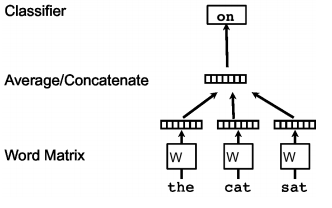
\includegraphics[height=0.2\textheight]{img/word2vec_skip_gram}
    \caption{Word2vec -- Skip gram architecture\cite{doc2vec}}
    \label{fig:word2vec_skip_gram}
\end{figure}

Other things to mention:
\begin{itemize}
    \item show 2D projection of vectors
    \item $king + woman - man = queen$
\end{itemize}

\subsection{Paragraph Vector (Doc2Vec)}
Explain doc2vec\cite{doc2vec}.

\begin{comment}
dbow
is a simpler model and ignores
word order, while
dmpv
is a more complex model
with more parameters

dbow 
works in the same way as skip-gram, except that the input is replaced by a special token representing the document (i.e. v_w_I is a vector rep-
resenting the document).  In this architecture, the order of words in the document is ignored; hence the name distributed bag of words.

dmpv
works in a similar way to cbow. For the input, dmpv introduces  an  additional  document token  in  addition  to  multiple  target  words. Unlike cbow, however, these vectors are not summed but concatenated (i.e.
v_w_I is a concatenated vector containing the document token and several target words). The objective is again to predict a context word given the concatenated document and word vectors..

\end{comment}

\begin{itemize}
    \item distributed memory version (dm) (\cref{fig:doc2vec_dm})
      \subitem small extension to cbow word2vec
      \subitem acts as a memory - what is missing from the current context?
    \item distributed bag of words (dbow) (\cref{fig:doc2vec_dbow})
      \subitem similar to skip-grams in word2vec
\end{itemize}

\begin{figure}[h]
	\centering
	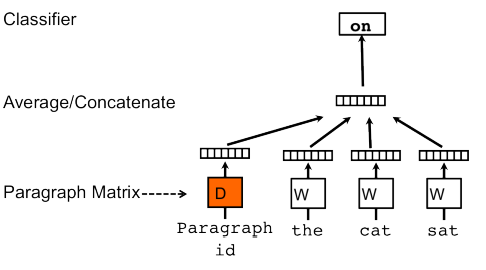
\includegraphics[height=0.2\textheight]{img/doc2vec_dm}
    \caption{Paragraph Vector -- Distributed Memory version\cite{doc2vec}}
    \label{fig:doc2vec_dm}
\end{figure}

\begin{figure}[h]
	\centering
	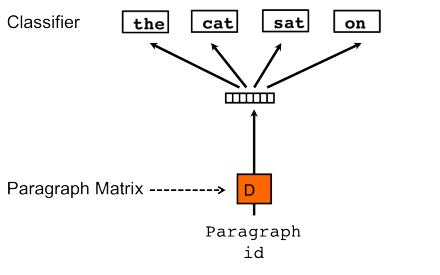
\includegraphics[height=0.2\textheight]{img/doc2vec_dbow}
	\caption{Paragraph Vector -- Distributed Bag of Words version\cite{doc2vec}}
	\label{fig:doc2vec_dbow}
\end{figure}

\subsection{Deep Learning}
deep learning\cite{Goodfellow}

Input - sequence of word embeddings.

\subsubsection{Recurrent Neural Network (RNN)}
\begin{itemize}
    \item cite relevant papers
    \item put an image of the network
    \item LSTM units
\end{itemize}

\subsubsection{Convolutional Neural Networks}
Show Yoon Kim's\cite{yoon_kim} architecture (\cref{fig:cnn_kim}).


Mention Zhang.\cite{cnn_zhang}.

\begin{figure}[h]
	\centering
	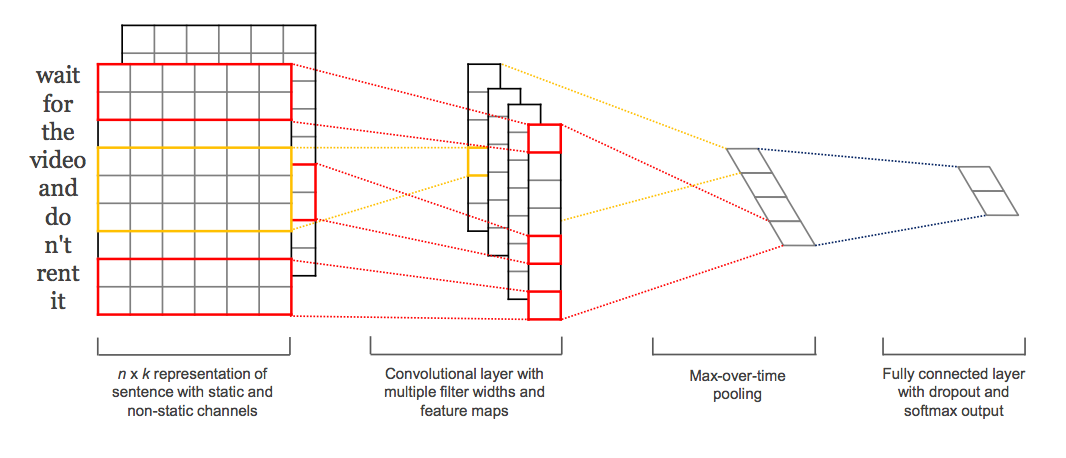
\includegraphics[height=0.2\textheight]{img/cnn_kim}
	\caption{Convolutional neural network with multiple filter sizes\cite{yoon_kim}}
	\label{fig:cnn_kim}
\end{figure}


%%%%%%%%%%%%%%%%%%%%%%%%%%%%%
%%%%%%%%% BOOSTING %%%%%%%%%%
%%%%%%%%%%%%%%%%%%%%%%%%%%%%%
\begin{comment}

\begin{itemize}
    \item Random Forest
    \item XGBoost
    \item stacking
\end{itemize}
\end{comment}



\begin{comment}
\subsection{Annoy}
Annoy\cite{annoy} is a algorithm developed by Erik Bernhardsson at Spotify, which enables quick search for the nearest neighbours. The drawback of the traditional kNN algorithm is its linear prediction time and huge amount of memory needed, which doesn't scale once we have hundreds of thousands data points.

Annoy uses random projections and recursively splits the space between two data points by a random hyperplane. All the splits are stored in the tree. The whole algorithm is run $n$ times to create $n$ trees. The more trees, the better the accuracy and slower the training and prediction time.
\end{comment}

\section{Project Gutenberg}
\begin{itemize}
    \item What is Project Gutenberg.
    \item How many books are there in Project Gutenberg
    \item What types (classes) of books
    \item Metadata for genre classification.
\end{itemize}

\chapter{Design}
Describing experiments and approaches of the thesis.
\section{Experiment 1}

\section{Experiment 2}

\chapter{Evaluation}

\chapter{Implementation}
Describes details of the implementations. We used gensim\cite{gensim}.
\begin{itemize}
  \item Which algorithm is used?
  \item How is it deployed? Flask, Heroku $\cdots$
\end{itemize}

\chapter{Summary}
\section{Summary and Conclusions}
\section{Future Work}


\include{epilog}

%%% Bibliography
%%% Bibliography (literature used as a source)
%%%
%%% We employ bibTeX to construct the bibliography. It processes
%%% citations in the text (e.g., the \cite{...} macro) and looks up
%%% relevant entries in the bibliography.bib file.
%%%
%%% The \bibliographystyle command selects, which style will be used
%%% for references from the text. The argument in curly brackets is
%%% the name of the corresponding style file (*.bst). Both styles
%%% mentioned in this template are included in LaTeX distributions.

% \bibliographystyle{plainnat}    %% Author (year)
\bibliographystyle{unsrt}     %% [number]

\renewcommand{\bibname}{Bibliography}

%%% Generate the bibliography. Beware that if you cited no works,
%%% the empty list will be omitted completely.

\bibliography{bibliography}

%%% If case you prefer to write the bibliography manually (without bibTeX),
%%% you can use the following. Please follow the ISO 690 standard and
%%% citation conventions of your field of research.

% \begin{thebibliography}{99}
%
% \bibitem{lamport94}
%   {\sc Lamport,} Leslie.
%   \emph{\LaTeX: A Document Preparation System}.
%   2nd edition.
%   Massachusetts: Addison Wesley, 1994.
%   ISBN 0-201-52983-1.
%
% \end{thebibliography}


%%% Figures used in the thesis (consider if this is needed)
%\listoffigures

%%% Tables used in the thesis (consider if this is needed)
%%% In mathematical theses, it could be better to move the list of tables to the beginning of the thesis.
%\listoftables

%%% Abbreviations used in the thesis, if any, including their explanation
%%% In mathematical theses, it could be better to move the list of abbreviations to the beginning of the thesis.
%\chapwithtoc{List of Abbreviations}

%%% Attachments to the bachelor thesis, if any. Each attachment must be
%%% referred to at least once from the text of the thesis. Attachments
%%% are numbered.
%%%
%%% The printed version should preferably contain attachments, which can be
%%% read (additional tables and charts, supplementary text, examples of
%%% program output, etc.). The electronic version is more suited for attachments
%%% which will likely be used in an electronic form rather than read (program
%%% source code, data files, interactive charts, etc.). Electronic attachments
%%% should be uploaded to SIS and optionally also included in the thesis on a~CD/DVD.
%%% Allowed file formats are specified in provision of the rector no. 72/2017.
\iffalse
\appendix
\chapter{Attachments}

\section{First Attachment}
\fi

\openright
\end{document}
